%
% fig-faserintegration.tex
%
% (c) 2025 Prof Dr Andreas Müller
%
\begin{figure}
\centering
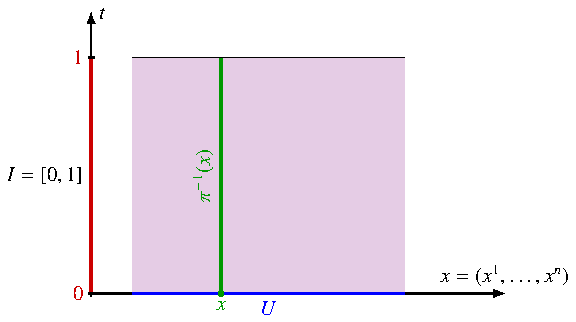
\includegraphics{chapters/060-pformen/images/faserintegration.pdf}
\caption{Die Projektion $\pi(x,t)=x$ projiziert die grünen Fasern
auf Punkte in $U$. Die Faserintegration integriert über solche Fasern
und reduziert damit den Grad einer $p+1$-Form auf $U\times [0,1]$
auf eine $p$-Form.
\label{buch:pformen:poincarelemma:fig:faserintegration}}
\end{figure}
